\documentclass{standalone}

\usepackage{tikz}
\usepackage{circuitikz}

\tikzset{block/.style = {draw, fill=white, very thick, rectangle, minimum height=1cm, minimum width=2cm},
         lblock/.style={draw,fill=white,very thick, rectangle, minimum height=3cm, minimum width=1cm},
         sum/.style= {draw, fill=white, very thick, circle, node distance=0.5cm}}

         
\begin{document}
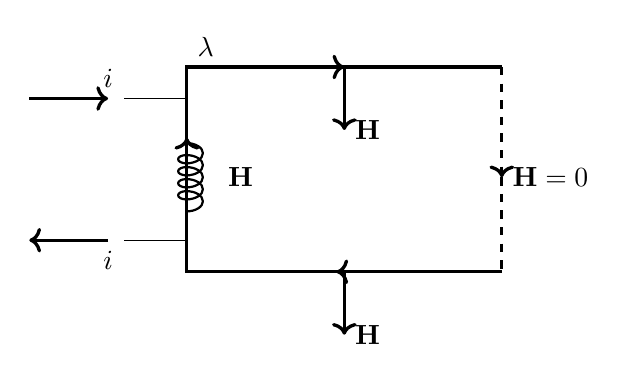
\begin{tikzpicture}[scale=2]

    \draw[-](0,1)--(-0.4,1);
    \draw[-](0,0.1)--(-0.4,0.1);
    \draw[->,very thick](-1,1)--(-0.5,1)node[above]{$i$};
    \draw[->,very thick](-0.5,0.1)node[below]{$i$}--(-1,0.1);

    \draw[-,very thick](2,1.2)--(0,1.2)node[above right]{$\lambda$}--(0,-0.1)--(2,-0.1);
    \draw[->,very thick](0.95,1.2)--(1,1.2);
    \draw[<-,very thick](0.95,-0.1)--(1,-0.1);
    \draw[dashed,->, very thick](2,1.2)--(2,0.5)node[right]{$\mathbf{H}=0$};
    \draw[dashed,very thick](2,0.5)--(2,-0.1);
    \draw[->,very thick](1,1.2)--(1,0.8)node[right]{$\mathbf{H}$};
    \draw[->,very thick](1,-0.1)--(1,-0.5)node[right]{$\mathbf{H}$};
    \draw[->,very thick](0,0.25)--(0,0.75);
    \node[right]at(0.2,0.5){$\mathbf{H}$};
    \draw(0,1)to[L](0,0);


\end{tikzpicture}
\end{document}